\section{Development of the First Feature (Login/Registration)}

The login and registration feature was the first developed in Part 1, and it illustrates the same prompt design, generation, review, refinement, and testing cycle that recurred throughout the rest of development. As the module responsible for authenticating users and scoping the rest of the application to a single logged-in user, it was also treated as a foundation the later feature work would depend on.

The frontend was developed first. Development began with a visual mockup of the login page, given to the agent together with an instruction to reproduce it as closely as possible; the agent was told in advance to ask clarifying questions before generating any code, and additional details not fully captured by the mockup itself --- specific colors, fonts, and layout choices --- were provided before generation started rather than left for the agent to infer. Styling was explicitly constrained to Bootstrap, backend integration was deliberately postponed so the page could first be built as a UI-only component, and non-essential elements such as a "Forgot password" link were left as placeholders. The agent was also not permitted to modify any existing file without asking first (\Cref{fig:login-mockup}).

\begin{figure}[H]
    \centering
    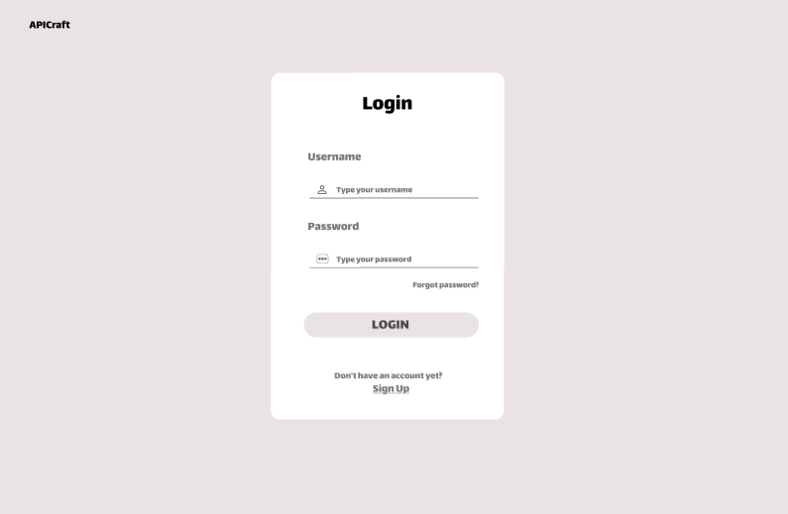
\includegraphics[width=0.55\linewidth]{Bilder/Part1-UnstructuredDevelopment/login_mockup.png}
    \caption{Mockup of the login page provided to the agent as the initial specification.}
    \label{fig:login-mockup}
\end{figure}

The first generated version matched the mockup closely in color and overall structure, but the login card was too narrow and sat too centered on the page, which did not match the intended design (\Cref{fig:login-initial-result}).

\begin{figure}[H]
    \centering
    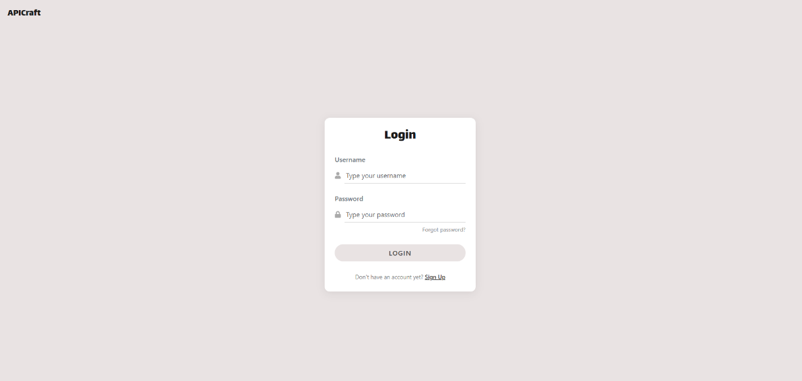
\includegraphics[width=0.55\linewidth]{Bilder/Part1-UnstructuredDevelopment/login_initial_result.png}
    \caption{First version of the login page generated by the agent, before layout adjustments.}
    \label{fig:login-initial-result}
\end{figure}

This was corrected through further prompts adjusting the card's width and the alignment of the input fields --- an iterative process in which the first output served as a starting point rather than a finished result (\Cref{fig:login-final-result}).

\begin{figure}[H]
    \centering
    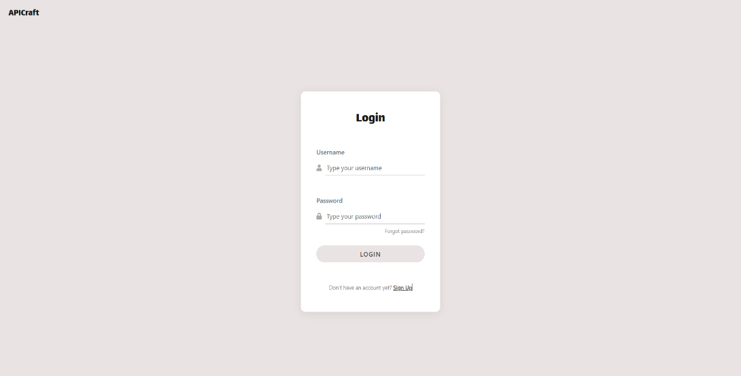
\includegraphics[width=0.55\linewidth]{Bilder/Part1-UnstructuredDevelopment/login_final_result.png}
    \caption{Login page after iterative refinement of card width and input field alignment.}
    \label{fig:login-final-result}
\end{figure}

Across these iterations, the agent occasionally introduced CSS rules or code that were not needed for the page to function, which had to be identified and manually removed. The sign-up page was then built using the same mockup-first workflow and the same constraints.

The backend was developed afterward, in a single prompt covering the data model, both endpoints, and the required behavior together. The prompt asked for a User model with an id, a username, and a password, a signup endpoint validating that both fields were provided and that the username was not already taken, and a login endpoint validating credentials against the stored data --- along with minimal frontend integration to connect to the pages already built and the same requirement not to modify existing files without permission. This prompt did not ask for an email field at all; the omission was only identified afterward, once the specification was reviewed against what the feature was actually meant to support, and a follow-up prompt added it to the model and to both endpoints.

Reviewing the resulting implementation surfaced two further problems, neither of which had been anticipated in the original prompt. First, the database did not enforce email uniqueness, so multiple users could register with the same email address --- a consequence of the original prompt never stating that the field should be constrained as unique. Second, the validation feedback returned to the user was too generic: both a missing username and a missing password produced the same message, "Username and password are required," rather than identifying which field was actually missing, and no distinct message existed for the case of an email that was already registered (\Cref{fig:signup-generic-validation}).

\begin{figure}[H]
    \centering
    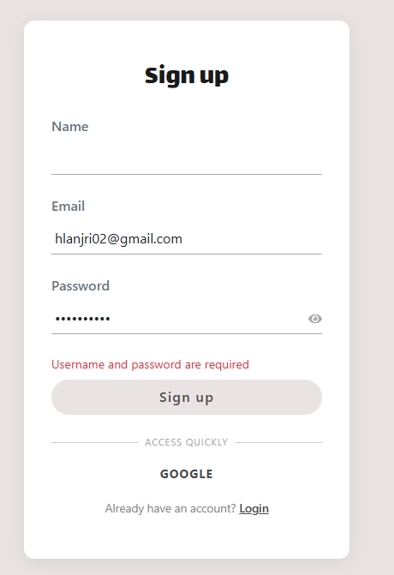
\includegraphics[width=0.35\linewidth]{Bilder/Part1-UnstructuredDevelopment/signup_generic_validation.png}
    \caption{Sign-up form displaying the generic validation message that did not identify which field was missing.}
    \label{fig:signup-generic-validation}
\end{figure}

Both were corrected through further prompts refining the backend validation logic and the corresponding frontend error handling, after which the messages returned distinguished a missing username, a missing password, and a duplicate email as separate cases.

Taken together, the missing email field, the missing uniqueness constraint, and the generic validation messages all trace back to the same cause: none of them were stated in the prompt that first specified the feature, and all three were only caught once the implementation was reviewed against what was actually intended rather than against what had literally been asked for.

